Nous créons un filtre passe bas de type Butterworth avec les caractéristiques suivantes:\\
\begin{itemize}
\item Fréquence d'échantillonnage : 8 kHz
\item Fréquence de coupure : 1 kHz
\item Largeur de transition : 200 Hz
\item Ondulation maximale dans la bande passante : 1 dB
\item Atténuation minimaledans la bande coupée : 40 dB
\end{itemize}
~\\
Les trois figures suivantes nous la réponse impulsionnelle, les pôles et les zéros ainsi que la fonction de transfert du filtre que nous avons créé.

\begin{figure}[H]
\centering
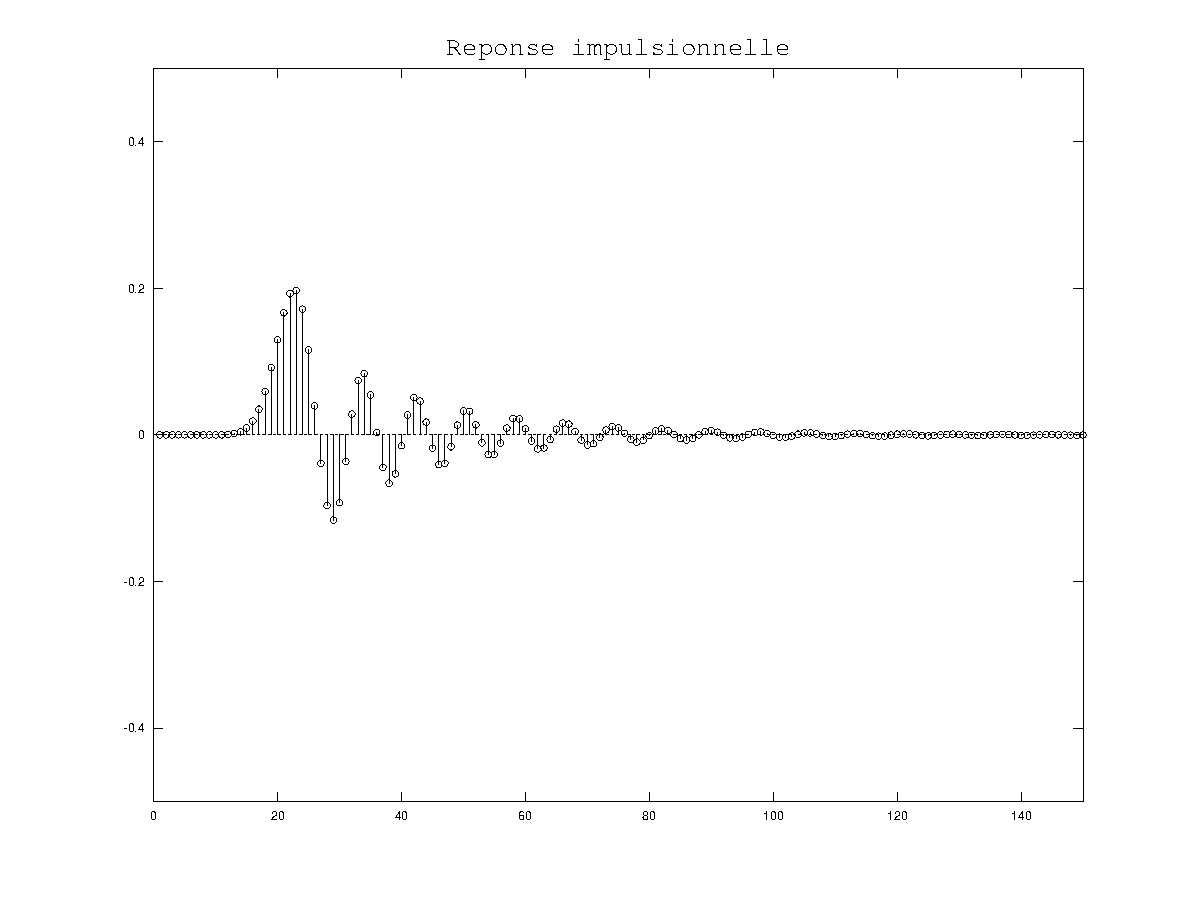
\includegraphics[width=9cm]{resEx4/repImpulsion.pdf}
\caption{Réponse impulsionnelle du filtre de Butterworth}
\end{figure}

\begin{figure}[H]
\centering
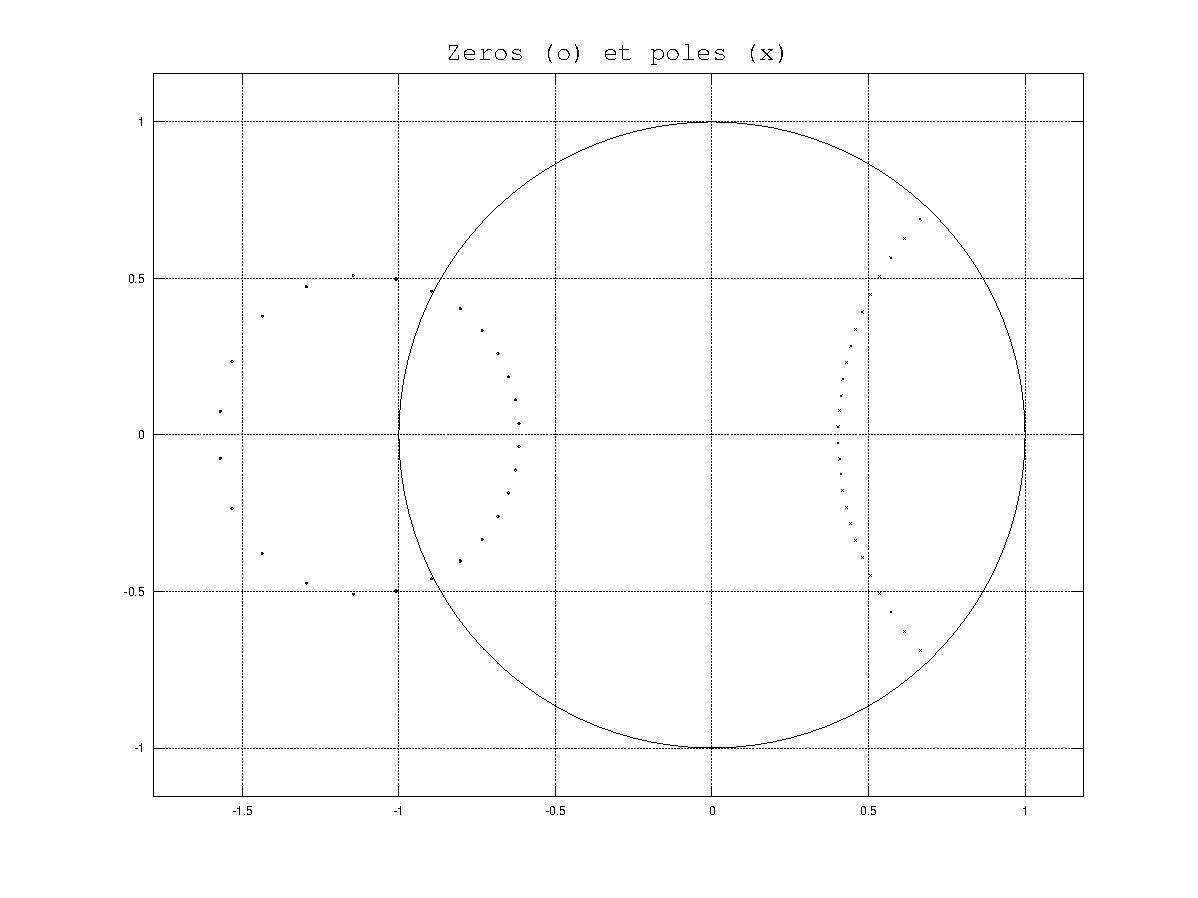
\includegraphics[width=9cm]{resEx4/ZP.pdf}
\caption{Les pôles et les zéros du filtre de Butterworth}
\end{figure}

\begin{figure}[H]
\centering
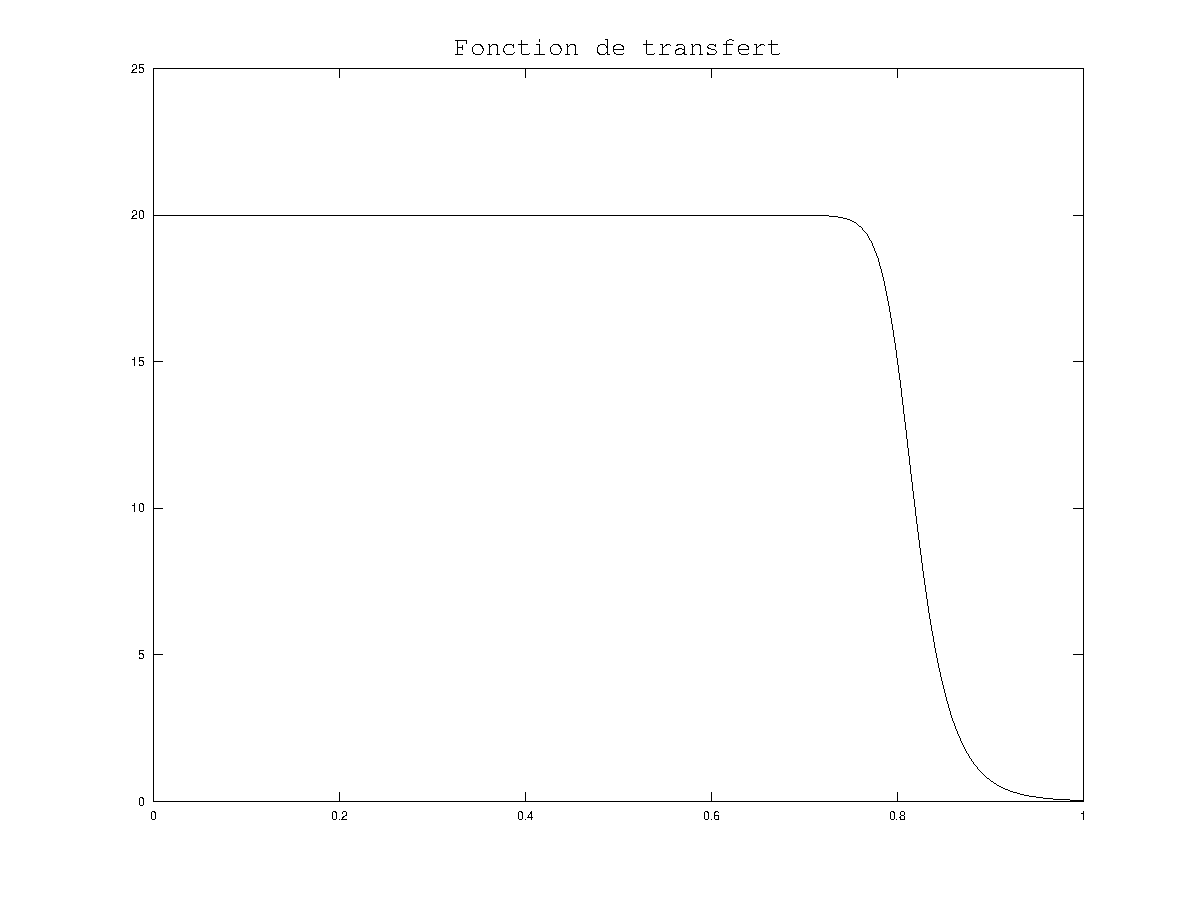
\includegraphics[width=9cm]{resEx4/fctTransfert.pdf}
\caption{Fonction de transfert du filtre de Butterworth}
\end{figure}

Le signal composé de deux sinusoïdes, une de fréquence 800 Hz et l'autre de fréquence 1.4kHz toutes deux échantillonnées à 8 kHz nous donne le signal suivant : 

\begin{figure}[H]
\centering
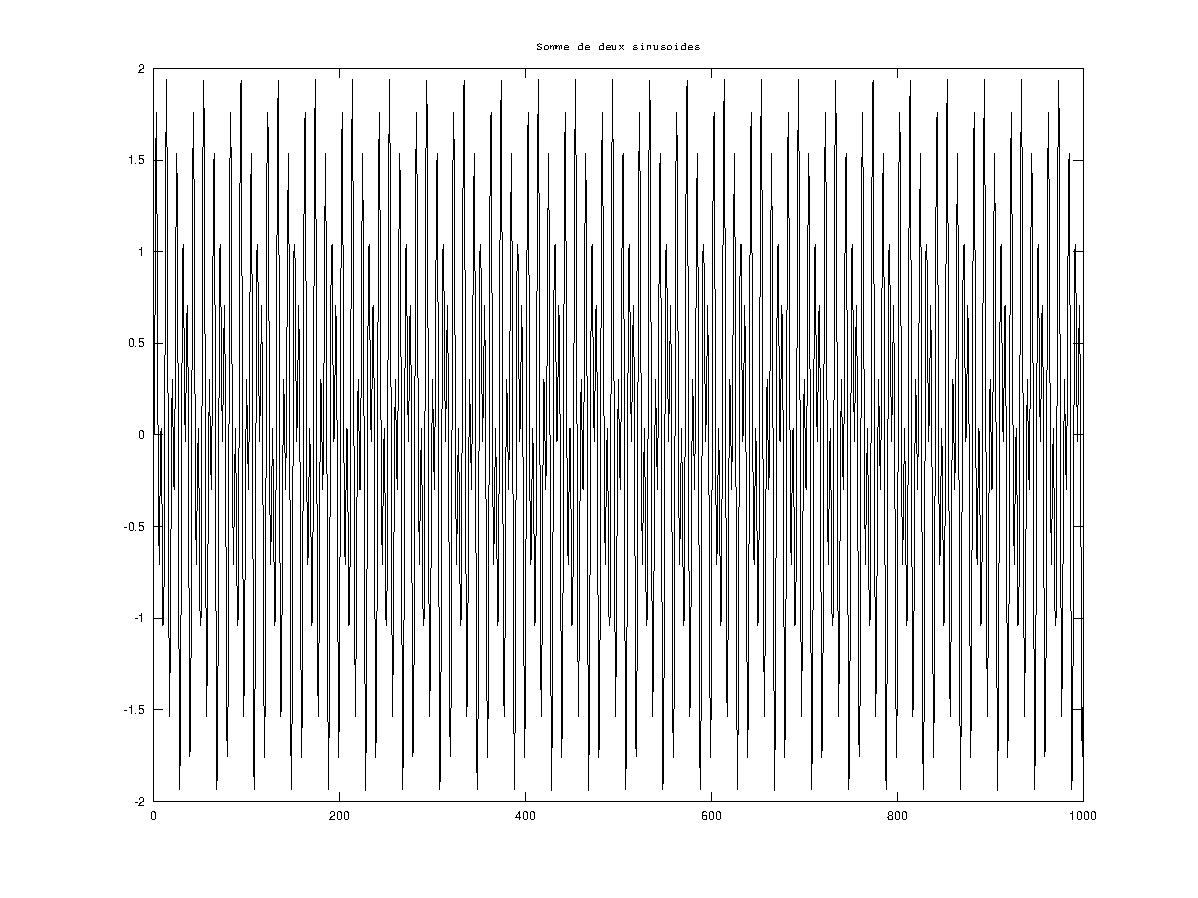
\includegraphics[width=9cm]{resEx4/2sin.pdf}
\caption{Signal formé de deux sinusoïdes}
\end{figure}

Le spectre de ce signal avant filtrage est représenté ci dessous:

\begin{figure}[H]
\centering
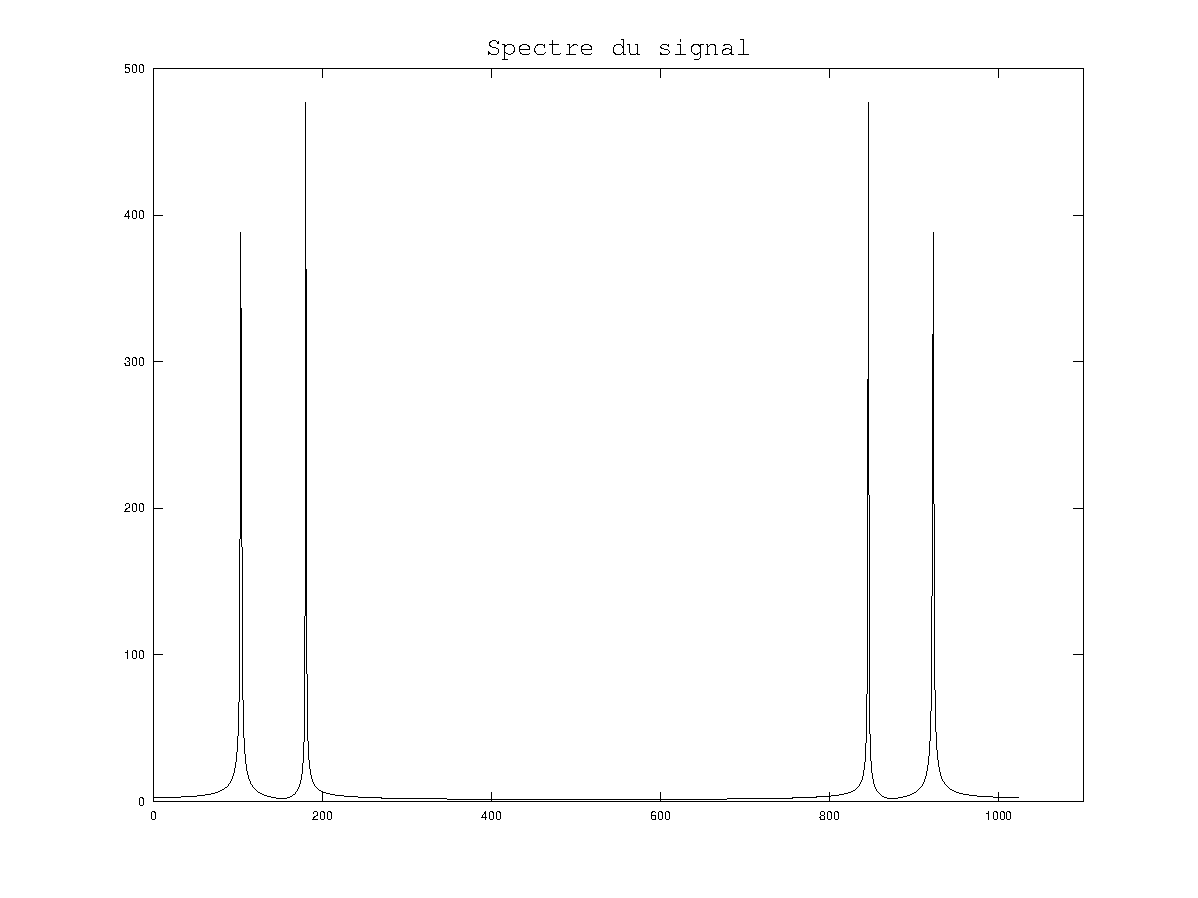
\includegraphics[width=9cm]{resEx4/spectreEntre.pdf}
\caption{Spectre d'entré}
\end{figure}

Une fois que nous lui avons appliqué le filtre nous obtenons:

\begin{figure}[H]
\centering
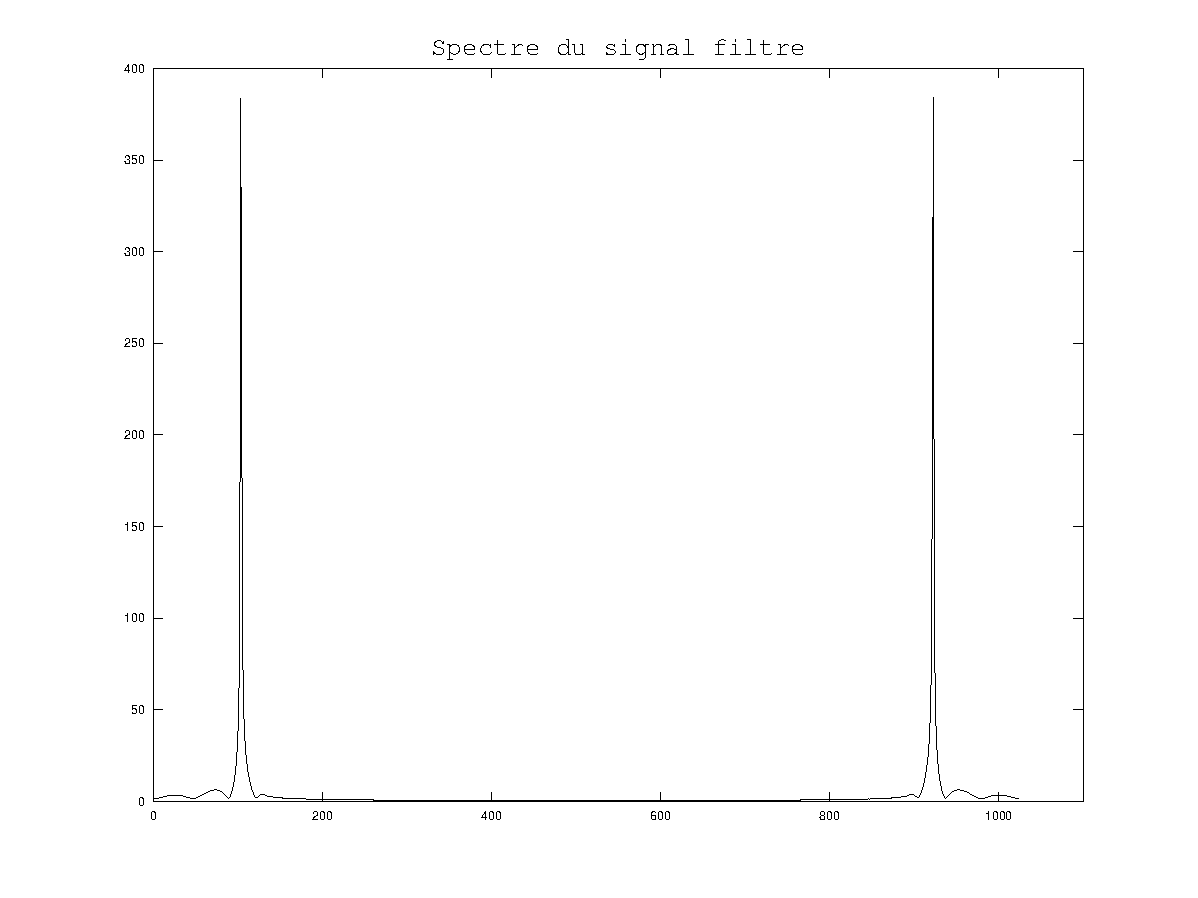
\includegraphics[width=9cm]{resEx4/spectreSortie.pdf}
\caption{Spectre de sortie}
\end{figure}
